% This is text associated with the open textbook "Open Electromagnetics"
% See immediately below for author, date
% This work is licensed under the Creative Commons Attribution-ShareAlike 4.0 International License. (CC BY-SA 4.0) 
% To view a copy of the license, visit http://creativecommons.org/licenses/by-sa/4.0/

%ORB TITLE Decomposition of a Wave into TE and TM Components
%ORB AUTHOR 0        # S.W. Ellingson, Virginia Tech (ellingson@vt.edu)
%ORB DATE 20191117   # yyyymmdd
%ORB ABSTRACT 

\label{m0166_Decomposition_into_TE_and_TM} % <-- Must match name of this file and module directory name.  Don't mess with this!
\index{transverse electric|(}
\index{transverse magnetic|(}

A broad range of problems in electromagnetics involve scattering of a plane wave by a planar boundary between dissimilar media.
Section~\ref{m0161_Waves_at_Planar_Boundary} (``Plane Waves at Normal Incidence on a Planar Boundary Between Lossless Media'') addressed the special case in which the wave arrives in a direction which is perpendicular to the boundary (i.e., ``normal incidence'').
Analysis of the normal incidence case is simplified by the fact that the directions of field vectors associated with the reflected and transmitted are the same (except possibly with a sign change) as those of the incident wave.  
For the more general case in which the incident wave is \emph{obliquely} incident (i.e., not necessarily normally-incident), the directions of the field vectors will generally be different.
This added complexity is easily handled if we take the effort to represent the incident wave as the sum of two waves having particular polarizations.  
These polarizations are referred to as \emph{transverse electric} (TE) and \emph{transverse magnetic} (TM).
This section describes these polarizations and the method for decomposition of a plane wave into TE and TM components.
We will then be prepared to address the oblique incidence case in a later section.

To begin, we define the ray-fixed coordinate system 
\index{ray-fixed coordinates}
shown in Figure~\ref{m0166_fRayFixedCoordinateSystemIncident}.
%
\begin{figure}[b!] % <--- "[b]" for first figure in section *only*; delete for 2nd and subsequent figures
\begin{center}
\pdftooltip{{  % note double braces
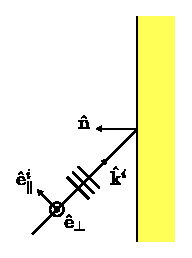
\includegraphics[width=0.4\columnwidth]{modules/m0166_fRayFixedCoordinateSystemIncident.eps} 
% https://commons.wikimedia.org/wiki/File:Coord_system_for_TE-TM_decomposition.svg
}}{Plane wave obliquely incident on a planar boundary described in a ray-fixed coordinate system}
\end{center}
\centerline{\scriptsize 
\copyright~\hyperref[m0166_fRayFixedCoordinateSystemIncident_Credit]{C.\ Wang} 
\href{https://creativecommons.org/licenses/by-sa/4.0/}{CC BY-SA 4.0} 
} % \centerline 
\caption{
\label{m0166_fRayFixedCoordinateSystemIncident}
Coordinate system for TE-TM decomposition.  Since both $\hat{\bf k}^i$ and $\hat{\bf n}$ lie in the plane of the page, this is also the plane of incidence.
}
\end{figure}
%
In this figure, 
$\hat{\bf k}^i$ is a unit vector indicating the direction in which the incident wave propagates.
The unit normal $\hat{\bf n}$ is perpendicular to the boundary, and points into the region from which the wave is incident.
We now make the following definition:
%
%%%%%%%%%%%%%%%%%%%%%%%%%%%%%%%%%%%%%%%%%%%%%%%
%ORB HIGHLIGHT
\begin{mdframed}[backgroundcolor=yellow!20,nobreak=true] 
The plane of incidence 
\index{plane of incidence}
is the plane in which \emph{both} the normal to the surface ($\hat{\bf n}$) and the direction of propagation ($\hat{\bf k}^i$) lie.    
\end{mdframed}
%%%%%%%%%%%%%%%%%%%%%%%%%%%%%%%%%%%%%%%%%%%%%%%
%
The TE-TM decomposition consists of finding the components of the electric and magnetic fields which are perpendicular (``transverse'') to the plane of incidence.
Of the two possible directions that are perpendicular to the plane of incidence, we choose $\hat{\bf e}_{\perp}$, defined as shown in Figure~\ref{m0166_fRayFixedCoordinateSystemIncident}.  
From the figure, we see that:
%
\begin{equation}
\hat{\bf e}_{\perp} \triangleq \frac{ \hat{\bf k}^i \times \hat{\bf n} }{ \left| \hat{\bf k}^i \times \hat{\bf n} \right| }
\label{m0166_eeperp}
\end{equation}
%
Defined in this manner, $\hat{\bf e}_{\perp}$ is a unit vector which is perpendicular to both $\hat{\bf k}^i$, and so may serve as a basis vector of a coordinate system which is attached to the incident ray.
The remaining basis vector for this ray-fixed coordinate system is chosen as follows:
%
\begin{equation}
\hat{\bf e}^i_{\parallel} \triangleq \hat{\bf e}_{\perp} \times \hat{\bf k}^i
\end{equation}
%
Defined in this manner, $\hat{\bf e}^i_{\parallel}$ is a unit vector which is perpendicular to both $\hat{\bf e}_{\perp}$ and $\hat{\bf k}^i$, and parallel to the plane of incidence.

Let us now examine an incident uniform plane wave in the new, ray-fixed coordinate system.
We begin with the following phasor representation of the electric field intensity:
%
\begin{equation}
\widetilde{\bf E}^i = \hat{\bf e}^i E_0^i e^{-j{\bf k}^i\cdot{\bf r}}
\label{m0166_Ei}
\end{equation}
%
where
$\hat{\bf e}^i$ is a unit vector indicating the reference polarization,
%\footnote{That is, the direction in which the $\widetilde{\bf E}^i$ vector points when the phase of the scalar component of $\widetilde{\bf E}^i$ is zero.}
$E_0^i$ is a complex-valued scalar,
and ${\bf r}$ is a vector indicating the position at which $\widetilde{\bf E}^i$ is evaluated.
We may express $\hat{\bf e}^i$ in the ray-fixed coordinate system of Figure~\ref{m0166_fRayFixedCoordinateSystemIncident} as follows:
%
\begin{flalign}
\hat{\bf e}^i &= \left(\hat{\bf e}^i\cdot\hat{\bf e}_{\perp}\right)\hat{\bf e}_{\perp} \nonumber \\
              &+ \left(\hat{\bf e}^i\cdot\hat{\bf e}^i_{\parallel}\right)\hat{\bf e}^i_{\parallel} \nonumber \\
              &+ \left(\hat{\bf e}^i\cdot\hat{\bf k}^i\right)\hat{\bf k}^i  
\end{flalign}
%
The electric field vector is always perpendicular to the direction of propagation, so $\hat{\bf e}^i\cdot\hat{\bf k}^i=0$.
This leaves:
%
\begin{equation}
\hat{\bf e}^i = \left(\hat{\bf e}^i\cdot\hat{\bf e}_{\perp}\right)\hat{\bf e}_{\perp} 
              + \left(\hat{\bf e}^i\cdot\hat{\bf e}^i_{\parallel}\right)\hat{\bf e}^i_{\parallel}   
\end{equation}
%
Substituting this expression into Equation~\ref{m0166_Ei}, we obtain:
%
\begin{equation}
\widetilde{\bf E}^i = \hat{\bf e}_{\perp} E_{TE}^i e^{-j{\bf k}^i\cdot{\bf r}}
                    + \hat{\bf e}^i_{\parallel} E_{TM}^i e^{-j{\bf k}^i\cdot{\bf r}}
\label{m0166_Ei2}
\end{equation}
%
where
%
\begin{flalign}
E_{TE}^i &\triangleq E^i_0~\hat{\bf e}^i\cdot\hat{\bf e}_{\perp} \\
E_{TM}^i &\triangleq E^i_0~\hat{\bf e}^i\cdot\hat{\bf e}^i_{\parallel}
\end{flalign}
%
The first term in Equation~\ref{m0166_Ei2} is the transverse electric (TE) component of $\widetilde{\bf E}^i$, so-named because it is the component which is perpendicular to the plane of incidence.
The second term in Equation~\ref{m0166_Ei2} is the transverse magnetic (TM) component of $\widetilde{\bf E}^i$.
The term ``TM'' refers to the fact that the magnetic field associated with this component of the electric field is perpendicular to the plane of incidence.  This is apparent since the magnetic field vector is perpendicular to both the direction of propagation and the electric field vector. 

Summarizing: 
%%%%%%%%%%%%%%%%%%%%%%%%%%%%%%%%%%%%%%%%%%%%%%%
%ORB HIGHLIGHT
\begin{mdframed}[backgroundcolor=yellow!20,nobreak=true] 
The TE component is the component for which $\widetilde{\bf E}^i$ is perpendicular to the plane of incidence.
\end{mdframed}
%%%%%%%%%%%%%%%%%%%%%%%%%%%%%%%%%%%%%%%%%%%%%%%
%%%%%%%%%%%%%%%%%%%%%%%%%%%%%%%%%%%%%%%%%%%%%%%
%ORB HIGHLIGHT
\begin{mdframed}[backgroundcolor=yellow!20,nobreak=true] 
The TM component is the component for which $\widetilde{\bf H}^i$ is perpendicular to the plane of incidence; i.e., the component for which $\widetilde{\bf E}^i$ is parallel to the plane of incidence.
\end{mdframed}
%%%%%%%%%%%%%%%%%%%%%%%%%%%%%%%%%%%%%%%%%%%%%%%
Finally, observe that the total wave is the sum of its TE and TM components.
Therefore, we may analyze the TE and TM components separately, and know that the result for the combined wave is simply the sum of the results for the TE and TM components. 

As stated at the beginning of this section, the utility of the TE-TM decomposition is that it simplifies the analysis of wave reflection.
This is because the analysis of the TE and TM cases is relatively simple, whereas direct analysis of the scattering of arbitrarily-polarized waves is relatively difficult.

Note that the nomenclature ``TE'' and ``TM'' is commonly but not universally used.  
Sometimes ``TE'' is referred to as ``perpendicular'' polarization, indicated using the subscript ``$\perp$'' or ``s'' (short for \emph{senkrecht}, German for ``perpendicular''). 
Correspondingly, ``TM'' is sometimes referred to as ``parallel'' polarization, indicated using the subscript ``$\parallel$'' or ``p.''

Also, note that the TE component and TM component are sometimes referred to as the TE \emph{mode} and TM \emph{mode}, respectively.  While the terms ``component'' and ``mode'' are synonymous for the single plane wave scenarios considered in this section, the terms are not synonymous in general.  For example, the wave inside a waveguide may consist of multiple unique TE modes which collectively comprise the TE component of the field, and similarly the wave inside a waveguide may consist of multiple unique TM modes which collectively comprise the TM component of the field.

Finally, consider what happens when a plane wave is normally-incident upon the boundary; i.e., when $\hat{\bf k}^i=-\hat{\bf n}$.  
In this case, Equation~\ref{m0166_eeperp} indicates that $\hat{\bf e}_{\perp}=0$, so the TE-TM decomposition is undefined.
The situation is simply that both ${\bf E}^i$ and ${\bf H}^i$ are already both perpendicular to the boundary, and there is no single plane that can be uniquely identified as the plane of incidence.
We refer to this case as \emph{transverse electromagnetic} (TEM).
%%%%%%%%%%%%%%%%%%%%%%%%%%%%%%%%%%%%%%%%%%%%%%%
%ORB HIGHLIGHT
\begin{mdframed}[backgroundcolor=yellow!20,nobreak=true] 
A wave which is normally-incident on a planar surface is said to be transverse electromagnetic (TEM) 
\index{transverse electromagnetic (TEM)}
with respect to that boundary.  There is no unique TE-TM decomposition in this case.
\end{mdframed}
%%%%%%%%%%%%%%%%%%%%%%%%%%%%%%%%%%%%%%%%%%%%%%%
The fact that a unique TE-TM decomposition does not exist in the TEM case is of no consequence, because the TEM case is easily handled as a separate condition (see Section~\ref{m0161_Waves_at_Planar_Boundary}).

\index{transverse electric|)}
\index{transverse magnetic|)}

